In this section, we formally introduce the language we will focus on for writing data analyses.  This is a simple loop language with some primitives for calling queries. \mg{I would just call the language {\tt Loop} language}. After defining the syntax of the language and showing an example, we will define its trace-based operational semantics. This is the main technical ingredient we will use to define program's adaptivity. We will conclude this section by discussing the limitation of this language with respect to static analysis for adaptivity.

\subsection{Syntax}
\label{subsec:loop-syntax}
\begin{figure}
\[
\begin{array}{llll}
%  \mbox{Arithmatic Operators} & \oplus_a & ::= & + ~|~ - ~|~ \times 
% %
% ~|~ \div \\  
%   \mbox{Boolean Operators} & \oplus_b & ::= & \lor ~|~ \land ~|~ \neg\\
%   %
%   \mbox{Relational Operators} & \sim & ::= & < ~|~ \leq ~|~ == \\  
%  \mbox{Label} & l & := & \mathbb{N} \\ 
%  \mbox{While Map} & w & \in & \mbox{Label} \times \mathbb{N} \\
\mbox{Arithmetic Expr.} & \aexpr & ::= & 
	%
	n ~|~ x ~|~ \chi ~|~ \aexpr \oplus_a \aexpr ~|~ [] ~|~ [\aexpr, \dots, \aexpr] \\
% \sep \pi (l , \aexpr, \aexpr) \\
    %
\mbox{Boolean Expr.} & \bexpr & ::= & 
	%
	\etrue ~|~ \efalse  ~|~ \neg \bexpr
	 ~|~ \bexpr \oplus_b \bexpr
	%
	~|~ \aexpr \sim \aexpr \\
\mbox{Expressions} & \expr & ::= & \aexpr \sep \bexpr \\	
\mbox{commands} & c & ::= &  \eskip  ~|~  \assign x \expr ~|~  \assign{x}{ q(e)}
%
~|~ \eloop ~ \aexpr  ~ \edo ~ c  ~|~ c;c  ~|~ \eif(\bexpr, c, c) 	 
	\\
%\mbox{Variables} & \mathcal{VAR}  & ::= & \{ {x} \} \\
%
% \mbox{Trace} & t & ::= & [] ~|~ [(q, v)^{(l, w) }] ~|~ t ++ t
\end{array}
\]
 \caption{Syntax of loop language}
    \label{fig:syntax_highlevel}
\end{figure}

We introduce the syntax of the {\tt Loop} language we will use to write our data analyses in Figure~\ref{fig:syntax_highlevel}.
%expression
It is standard that expressions can be either arithmetic expressions or boolean expressions.
An arithmetic expression can be a  constant $n$ denoting integer, a variable $x$ from some countable set $\tt Var$, the special variable $\chi$ representing a row of the database, a combination of arithmetic expressions by means of the symbol $\oplus_a$, denoting basic operations including addition, product, subtraction, etc., the empty list $[]$, a list $[a_1,\ldots,a_k]$ of arithmetic expressions.
%
A boolean expression can be {\tt true} or {\tt false}, the negation of
a boolean expression, or a combination of boolean expressions by means of $\oplus_b$, denoting basic boolean connectives, or the result of some basic comparison $sym$ between arithmetic expressions, e.g. $\leq,=,<,$ etc. 
% 
%
  A command $c$ can either be $\eskip$, an assignment command $\assign{x}{\expr}$, the composition of two commands $c;c$, an if statement $\eif(\bexpr, c, c)$, a loop statement  $\eloop ~ \aexpr ~ \edo ~ c $.
 
 The main novelty of the syntax is the query request command $\assign{x}{q(\expr)}$. As a reminder, the aforementioned tight bound of adaptive data analysis in Section\ref{sec:overview} focuses on linear queries. So our framework targets the linear queries as well. The linear query is specified by a function from rows to $[0,1]$ or $[-1,+1]$. To express these functions, we introduce the special variable $\chi$ to represent the rows of the database in the arithmetic expressions. In this sense, a simple linear query which returns the first element of the row is written as $q(\chi(1))$, as a notation for a query $q(\chi) = \chi(1)$.  
 
 
% The query $q(\expr)$ in this command is abstract, and the expression $\expr$ inside the query stores the information of the elements used during the construction of the query. This kind of abstraction of query helps in our analysis and still remain expressive enough for adaptive analysis algorithms. 


\mg{I don't think that this corresponds exactly to our approach. I think that we want to focus on linear queries, these are the ones for which we have the bounds. A linear query is specified by a function from rows to [0,1] or [-1,+1]. So, in some sense, we want to have a language that describes these functions. Cannot we use $q(r)=e$ where $r$ is a special variable denoting the given row, and $e$ is an expression as we have right now? Example: $q_j(x)=x(i)\cdot x(j)$ can be written as $q(\chi (i)\cdot \chi (j))$ which is a notation for
$q=\lambda \chi \chi (i)\cdot \chi (j)$.}

  We have seen a simplified version of the two round algorithm in Section~\ref{sec:overview}. We show its complete version $TRC$ expressed in our loop language on the left hand side in Figure~\ref{fig:tworound_complete}.
 
 
 
 
%  \subsection{An example}
%  \mg{I will not change this section because I think we need to think more about what our language of queries is. As I said above, I think we should be more explicit. For example, I would write $q_1$ as $q(x[j]\cdot x[i])$ or something similar. I also don't think it is a good idea to present Algorithm~\ref{alg:two_round} first, and then show how to write this in our language. We can use two-rounds to introduce our language but I would present it directly in our language without the algorithm. I see several issues in using the algorithm: first, you need to present the example twice, first for the algorithm and then the program; second, the algorithms is not much more real world than other examples - we took it from a research paper which actually now put it in the appendix. I suggest we present the example but only as an example, withouth the algorithm.}

%  We go through a real-world adaptive data analysis algorithm in Algorithm~\ref{alg:two_round}, and see how our high level loop language expresses it. 
 

 
%  \begin{algorithm}
% \caption{A two-round analyst strategy for random data}
%  \label{alg:two_round}
% \begin{algorithmic}
% \REQUIRE Mechanism $\mathcal{M}$ with a hidden state $X\in \{-1,+1\}^{n\times (k+1)}$.
% \STATE  {\bf for}\ $j\in [k]$\ {\bf do}.  
% \STATE \qquad {\bf define} $q_j(x)=x(j)\cdot x(k)$ where $x\in \{-1,+1\}^{k+1}$.
% \STATE \qquad {\bf let} $a_j=\mathcal{M}(q_j)$ 
% \STATE \qquad \COMMENT{In the line above, $\mathcal{M}$ computes approx. the exp. value  of $q_j$ over $X$. So, $a_j\in [-1,+1]$.}
% \STATE {\bf define} $q_{k+1}(x)=\mathrm{sign}\big (\sum_{i\in [k]} x(i)\times\ln\frac{1+a_i}{1-a_i} \big )$ where $x\in \{-1,+1\}^{k+1}$.
% \STATE\COMMENT{In the line above,  $\mathrm{sign}(y)=\left \{ \begin{array}{lr} +1 & \mathrm{if}\ y\geq 0\\ -1 &\mathrm{otherwise} \end{array} \right . $.}
% \STATE {\bf let} $a_{k+1}=\mathcal{M}(q_{k+1})$
% \STATE\COMMENT{In the line above,  $\mathcal{M}$ computes approx. the exp. value  of $q_{k+1}$ over $X$. So, $a_{k+1}\in [-1,+1]$.}
% \RETURN $a_{k+1}$.
% \ENSURE $a_{k+1}\in [-1,+1]$
% \end{algorithmic}
% \end{algorithm}
As described before, the complete version still has two steps. The query asked in the first step now depends on the iteration number so that the query ask at the $j$ iteration is ($q_j(x) = x(j)\cdot x(k)$), expressed as $q(\chi(j)\cdot \chi(k))$. The iteration counter is initialized to 0, $j = 0$. In the second step, the final query is more complicated. It uses an auxiliary function   $\mathrm{sign}(y)=\left \{ \begin{array}{lr} +1 & \mathrm{if}\ y\geq 0\\ -1 &\mathrm{otherwise} \end{array} \right . $ The input of this function is $\sum_{i\in [k]} \chi(i)\times\ln\frac{1+a[i]}{1-a[i]}$, which sums the product of $\chi(i)$ and $\ln\frac{1+a[i]}{1-a[i]}$ that uses the value at index $i$ of the list $a$.
\begin{figure}
\[
{
\begin{array}{l}
\bf{TRC}(k) \\
    % \left[j \leftarrow 0 \right]^1 ; \\
    \\
   \clabel{ a \leftarrow []}^{1} ; \\
    \clabel{\assign{j}{0} }^{2} ; \\
    \eloop ~ \clabel{k}^{3} ~ \edo ~ \\
    \Big(
     \clabel{x \leftarrow q(\chi(j)\cdot \chi(k)) }^{4}  ; \\
     \clabel{\assign{j}{j+1}}^{5} ;\\
    \clabel{a \leftarrow x :: a}^{6}       \Big);\\
    \clabel{l \leftarrow q(\mathrm{sign}\big (\sum_{i\in [k]} \chi(i)\times\ln\frac{1+a[i]}{1-a[i]} \big ))}^{7}\\
\end{array} ~~
{
\begin{array}{l}
\bf{TRC^{ssa}}(k) \\
    % \left[j \leftarrow 0 \right]^1 ; \\ 
    \\
    \clabel{a_1 \leftarrow []}^{1} ; \\
    \clabel{\assign{j_1}{0} }^{2} ; \\
    \eloop ~ \clabel{k}^{3}, 0, ~ \edo [(j_3, j_1,j_2),(a_3, a_1,a_2)]~ \\
    \Big(
    \clabel{ x_1 \leftarrow q(\chi(j_3)\cdot \chi(k))}^{4}  ; \\
    \clabel{ \assign{j_2}{j_3+1} }^{5} ;\\
    \clabel{a_2 \leftarrow x_1 :: a_3}^{6}       \Big);\\
    \clabel{l_1 \leftarrow q(\mathrm{sign}\big (\sum_{i\in [k]} \chi(i)\times\ln\frac{1+a_3[i]}{1-a_3[i]} \big ))}^{7}\\
\end{array}
}
}
\]  
    \caption{Two round algorithm complete version}
    \label{fig:tworound_complete}
\end{figure}
% The second step of the Algorithm~\ref{alg:two_round} is to use the previous results $a_j$ from mechanism $\mathcal{M}$ for $j \in [k]$ to construct a complicated query $q_{k+1}$. In the high level language, we abstract this complex query as $q_2(a)$, $q_2$ representing queries of this complex kind of form and the argument $a$ is what we need for our analysis.

In a word, we go through a two-round adaptive analysis algorithm and shows how we can represent it in the loop language. It reveals the expressiveness of this language for most of adaptive data analysis algorithms. 

\subsection{ Trace-based Operational semantics}
In order to capture the dependency relations between queries we will evaluate programs in our {\tt Loop} language by means of a trace-based operational semantics. For distinguishing among different (occurrences of) queries, our trace-based semantics will generate traces that record also the line and loop numbers for different queries. For this reason we will consider a labelled version of the {\tt Loop} language. This can be described as follows:
% syntax
\mg{Change "while map" to "Loop maps" everywhere.}
\[
\begin{array}{llll}
 \mbox{Label} & l & := & \mathbb{N} \\ 
 \mbox{Loop Maps} & w & \in & \mbox{Label} \times \mathbb{N} \\
\mbox{Labelled commands} & c & ::= &   [\assign x \expr]^{l} ~|~  [\assign x q(e)]^{l}
 ~|~  \eloop ~ [\aexpr]^{l} ~ \edo ~ c  ~|~ c;c  ~|~ \eif([\bexpr]^l, c, c) 	 ~|~ [\eskip]^{l} \\
% 	\\ ~|~ [\eswitch( \expr, x, v_i \to  q_i)]^{l}
	%
% \mbox{Binary Operation} & \bop & ::= & + ~|~ - ~|~ \times 
% %
% ~|~ \div ~|~ < ~|~ \leq ~|~ = \\
% %
% \mbox{Unary Operation} & \uop & ::= & \ln ~|~ - \\
% %
% \mbox{Memory} & m & ::= & \emptyset ~|~ (x \to v) :: t \\
%
\mbox{Memory} & m & ::= & [] ~|~ m[x \to v] \\
\mbox{Trace} & t & ::= & [] ~|~ q(v)^{(l, w) } :: t \\
\mbox{Annotated Query} & \mathcal{AQ}  & ::= & \{ q(v)^{(l,w)}  \}
\end{array}
\]

The commands are now labelled --- we assume that labels are unique and correspond to the line of code where they appear. We denote the label $l$, which is the natural number standing for the line number of command in a program. Here, we put the label $l$ to the conditional $\bexpr$ in the if statement and to the loop counter $\aexpr$ in the loop command, which is helpful when we present the Loop Maps $w$.  
% implicitly this gives us a control flow graph representation for the program,
% which is useful when we define adaptivity in the later section. 
% t, m, w, explanation

A memory is standard, a map from variables to values. 
% \mg{I suggest to move the definitions of memories to the section on semantics.}
  An important component of the labelled loop language is $w$, what we call "Loop Maps", designed for loop specifically as an complementary annotation to the label. With the label and Loop Maps defined, we can show annotated queries $ \mathcal{AQ}$ have unique annotations.
  
 A trace $t$ is supposed to accumulate along with the execution of the program, it is
a list of annotated queries $ \mathcal{AQ}$, in which the query $q(v)$ has the unique annotation $(l,w)$. We can understand the annotation in such a way. The label $l$ locates arbitrary query request when we look at the execution path of a program with no loop. However, when loop repeats queries in its body, these query requests from varied iterations share the same line number. Hence, the label $l$ is not enough to distinguish queries in loops. For this purpose, another symbol is needed to represent the iteration number of a loop.
A simplified approach is to use natural number $n$ for the iteration number so that a pair $(l, n)$ can help, but it fails to support nested loop. This accounts for the appearance of loop maps $w$ into the annotation $(l,w)$. As a map from label $l$ to the iteration number n (a natural number), $w$ gives accurate information on which loop specified by its label and which iteration $n$ the query belongs to. We define some operations on $w$ below.
\[
\begin{array}{lll}
w \setminus l     & = w  & l \not\in Keys(w)   \\
     & = w_l & Otherwise \\
w + l & = w[l \to 1] & l \not \in Keys(w) \\   
     & = w [l \to w(l)+1] & Otherwise
\end{array}
\]
We denote $w \setminus l$ to remove the mapping of the key $l$ in the loop maps $w$, used when exiting the loop at the line $l$. We register a label to $w$ in the first iteration of a loop marked by label $l$ and assign $l$ to iteration $1$, and increase its iteration number by one mapped by the label $l$ when going into another iteration of the loop at line $l$. We denote $Keys(w)$ to return all the keys of the loop maps $w$.


A trace can be regarded as the history of query requests during the execution, generated by the trace-based small-step operational semantics. The evaluation of labelled commands are presented in Figure~\ref{fig:evaluation}, of the form $ \config{m,c, t, w} \to \config{m', \eskip, t', w'} $, stating a configuration $\config{m, c, t,w}$ evaluates to another configuration with the trace and while map updated and the command $c$ evaluated to $\eskip$. The configuration contains a memory $m$, a starting trace $t$, a starting while map $w$. Most of the time, the while map remains empty until the evaluation goes into the loop. We also have the evaluation of arithmatic expressions $\config{m,\aexpr} \aarrow \aexpr' $, evaluating an arithmatic expression $\aexpr$ in the memory $m$, and similar for the boolean expressions $\config{m, \bexpr} \barrow \bexpr'$.   

% figure, evaluation rules.
\begin{figure}
    \begin{mathpar}
% \boxed{ \config{m,\aexpr} \aarrow \aexpr' \, : \, Memory  \times AExpr \Rightarrow AExpr }
% \\
% \inferrule{ 
%  w(l) = 0
% }{
%  \config{m, w, f(l, \aexpr_1, \aexpr_2)} \aarrow \aexpr_1
% }
% %
% \and
% %
% \inferrule{
%  w(l) >0
% }{
%  \config{m, w, f(l, \aexpr_1, \aexpr_2)} \aarrow \aexpr_2
% }
% %
% \and
% %
% \inferrule{
%   \config{m, \aexpr_1 } \aarrow \aexpr_1'
% }{
%  \config{m, \aexpr_1 *_a \aexpr_2 } \aarrow \expr_1' *_a \aexpr_2
% }
% %
% \and
% %
% \inferrule{
%   \config{m, \aexpr_2 } \aarrow \aexpr_2'
% }{
%  \config{m, n_1 *_a \aexpr_2 } \aarrow n_1 *_a \aexpr_2'
% }
% %
% \and
% %
% \inferrule{
% n_3 = n_1 *_a n_2
% }{
%  \config{m, n_1 *_a n_2 } \aarrow n_3
% }
% \end{mathpar}
% % \vfill \pagebreak

% %
% \begin{mathpar}
% \boxed{ \config{m, \bexpr} \barrow \bexpr' \, : \, Memory \times BExpr \Rightarrow BExpr }
% \inferrule{
% }{
%  \config{m, \etrue} \barrow \etrue
% }
% %
% \and
% %
% \inferrule{
% }{
%  \config{m, \efalse} \barrow \efalse
% }
% %
% \and
% %
% \inferrule{
%   \config{m, \aexpr_1 } \aarrow \aexpr_1'
% }{
%  \config{m, \aexpr_1 *_r \aexpr_2 } \barrow \expr_1' *_r \aexpr_2
% }
% %
% \and
% %
% \inferrule{
%   \config{m, \aexpr_2 } \aarrow \aexpr_2'
% }{
%  \config{m, n_1 *_r \aexpr_2 } \barrow n_1 *_r \aexpr_2'
% }
% %
% \and
% %
% \inferrule{
% b_3 = n_1 *_r n_2
% }{
%  \config{m, n_1 *_r n_2 } \barrow b_3
% }
% %
% \and
% %
% \inferrule{
%  \config{m, \bexpr_1  } \barrow \bexpr_1' 
% }{
%  \config{m, \bexpr_1 *_b \bexpr_2 } \barrow \bexpr_1' *_b \bexpr_2
% }
% %
% \and
% %
% \inferrule{
%  \config{m, \bexpr_2  } \barrow \bexpr_2' 
% }{
%  \config{m, \etrue *_b \bexpr_2 } \barrow \etrue *_b \bexpr_2'
% }
% %
% \and
% %
% \inferrule{
%  \config{m, \bexpr_2  } \barrow \bexpr_2' 
% }{
%  \config{m, \efalse *_b \bexpr_2 } \barrow \efalse *_b \bexpr_2'
% }
% %
% \and
% %
% \inferrule{
%  \config{m, \bexpr  } \barrow \bexpr' 
% }{
%  \config{m, \neg \bexpr } \barrow \neg \bexpr'
% }
\end{mathpar}
%
\begin{mathpar}
\boxed{ \config{m, c, t,w} \xrightarrow{} \config{m', c',  t', w'} \; }
\and
% {  Memory \times Com  \times Trace \times WhileMap \Rightarrow^{} Memory \times Com  \times Trace \times WhileMap}
\inferrule
{
\config{m,\expr} \to \expr'
}
{
\config{m, [\assign{x}{q(\expr)}]^l, t, w} \xrightarrow{}  \config{m, [\assign{x}{q(\expr')}]^l, t, w}
}
~\textbf{low-query-e}
\and
\inferrule
{
q(v) = v_q
}
{
\config{m, [\assign{x}{q(v)}]^l, t, w} \xrightarrow{} \config{m[ v_q/ x], \eskip,  t \mathrel{++} [q(v)^{(l,w )}],w }
}
~\textbf{low-query-v}
%
%
% \inferrule
% {
% q(D) = v \and v \neq v'
% }
% {
% \config{m, \assign x q^*, D} \Rightarrow^{[(q, v')]} \config{m[x \to v'], \eskip, D}
% }
% ~\textbf{query}^*
% %
% \and
% %
% \inferrule
% {
% m, \expr \Rightarrow \expr'
% }
% {
% \config{m, [\assign{x}{ \expr}]^{l}, t,w} \xrightarrow{} \config{m, [\assign{x}{ \expr'}]^{l} , t,w}
% }
% ~\textbf{assn1}
%
\and
%
\inferrule
{
}
{
\config{m, [\assign x v]^{l},  t,w} \xrightarrow{} \config{m[v/x], [\eskip]^{l}, t,w}
}
~\textbf{low-assn}
%
\and
%
\inferrule
{
\config{m, c_1,  t,w} \xrightarrow{} \config{m', c_1',  t',w'}
}
{
\config{m, c_1; c_2,  t,w} \xrightarrow{} \config{m', c_1'; c_2, t',w'}
}
~\textbf{low-seq1}
%
\and
%
\inferrule
{
}
{
\config{m, [\eskip]^{l} ; c_2,  t,w} \xrightarrow{} \config{m, c_2,  t,w}
}
~\textbf{low-seq2}
%
\and
%
\inferrule
{
\config{ m, \bexpr} \barrow \bexpr'
}
{
\config{m, [\eif(\bexpr, c_1, c_2)]^{l},  t,w} 
\xrightarrow{} \config{m,  [\eif(\bexpr', c_1, c_2)]^{l},  t,w}
}
~\textbf{low-if}
%
\and
%
\inferrule
{
}
{
\config{m, [\eif(\etrue, c_1, c_2)]^{l},t,w} 
\xrightarrow{} \config{m, c_1,  t,w}
}
~\textbf{low-if-t}
%
\and
%
\inferrule
{
}
{
\config{m, [ \eif(\efalse, c_1, c_2)]^{l},  t,w} 
\xrightarrow{} \config{m, c_2,  t,w}
}
~\textbf{low-if-f}
% %
% \and
% %
% {\inferrule
% {
% }
% {
% \config{m, \ewhile([\bexpr]^l, c),  t,w} 
% \xrightarrow{} \config{m,  \eunfold{[\bexpr^{l}] }{\ewhile([\bexpr]^l,   c)} ,  t,w}
% }
% ~\textbf{while} }
% %
% \and
% %
% {\inferrule
% {
% \config{m, \bexpr} \rightarrow \bexpr'
% }
% {
% \config{m, \eunfold{[\bexpr]^l}{ c}, D, t,w} 
% \xrightarrow{} \config{m, \eunfold{[\bexpr']^l}{ c}, D, t,  w  }
% }
% ~\textbf{unfold}}
% %
% \and
% %
% {\inferrule
% {
% }
% {
% \config{m, \eunfold{[\efalse]^l}{c}, D, t,w} 
% \xrightarrow{} \config{m, [\eskip]^{l}, D, t,  (w \setminus l) }
% }
% ~\textbf{unfold-f}}

% \and
% %
% {\inferrule
% {
% }
% {
% \config{m, \eunfold{[\etrue]^l}{ c}, D, t,w} 
% \xrightarrow{} \config{m, c, D, t, (w+l) }
% }
% ~\textbf{unfold-t} }
% %
% \and
% %
% {
% \inferrule
% {
%   \config{m, \expr } \xrightarrow{} \expr'
% }
% {
% \config{m, [\eswitch(\expr, x, (v_i \to q_i))]^{l},  t,w} 
% \xrightarrow{} \config{m, [ \eswitch(\expr',x, (v_i \to q_i))]^{l},  t, w }
% }
% ~\textbf{switch}
% }
% %
% \and
% %
% {
% \inferrule
% {
% \empty
% }
% {
% \config{m, [ \eswitch(v_k,x, (v_i \to q_i))]^{l},  t,w} 
% \xrightarrow{} \config{m,  [\assign x q_k]^{l},  t, w }
% }
% ~\textbf{low-switch-v}
% }
% % %
% \and
% %
% {\inferrule
% {
% \config{m, \expr_N \xrightarrow{} \expr_N'  }
% }
% {
% \config{m,  \eloop ~ [\expr_N]^{l} ~ (f) ~ \edo ~ c ,  t, w }
% \xrightarrow{} \config{m, [ \eloop ~ [\expr_N]^{l} ~ (f) ~ \edo ~ c]^{l} ,  t, w }
% }
% ~\textbf{loop}
% }
%
\and
%
{\inferrule
{
 \valr_N > 0
}
{
\config{m, [\eloop ~ \valr_N  ~ \edo ~ c]^{l} ,  t, w }
\xrightarrow{} \config{m, c ;  [\eloop ~ (\valr_N-1) ~ \edo ~ c ]^{l},  t, (w + l) }
}
~\textbf{low-loop}
}
%
\and
%
{
\inferrule
{
 \valr_N = 0
}
{
\config{m,  [\eloop ~ \valr_N ~ \edo ~ c ]^{l} ,  t, w }
\xrightarrow{} \config{m, [\eskip]^{l} ,  t, (w \setminus l) }
}
~\textbf{low-loop-exit}
}
%
\end{mathpar}
    \caption{Trace-based Operational semantics}
    \label{fig:evaluation}
\end{figure}

% explanation of rules
The rule $\textbf{low-query-e}$ evaluates the argument of a query request. After the query arguments in the normal form, the rule $\textbf{low-query-v}$ modifies the starting memory $m$ to $m[v_q/x]$ using the return results $v_q$ of the query $q(v)$ request from a hidden database protected by a mechanism. We also notice that the trace expands by appending this query request $q(v)$ with the current annotation $(l,w)$. The rule for assignment is standard and the trace remains unchanged. The sequence rule keeps tracking the modification of the trace, and the evaluation rules for if conditional goes into one branch based on the result of the conditional $\bexpr$. The rules for loop are interesting. In rule $\textbf{low-loop}$, the while map $w$ is updated by $w + l$ because the execution goes into another iteration when $v_N >0$. When $v_N$ reaches $0$, the loop exits and the while map $w$ eliminates the label $l$ of this loop command by $w \setminus l$ in the rule $\textbf{low-loop-exit}$.     


\subsection{ Query-based may-dependency graph}
we give our attempt to define the number of rounds of adaptivity in our loop language, through a query-based dependency graph. A query-based dependency graph of a program consists of nodes, which are the queries during the execution of the program, and directed edges showing "may dependency" between two nodes(queries).


To this end, the definition of one query may depend on the other is fundamental to construct the query-based dependency graph. We first look at two possible candidates:
\begin{enumerate}
    \item One query depends on the other if and only if the change of the return results of one query may also change the results of the other query.
    \item One query depends on the other if and only if the change of the return results of one query may also change the appearance of the other query.
\end{enumerate}
   The first one looks reasonable to witnessing the result of one query according to the change of return result of another query. We can easily find that the two queries have nothing to do with each other in a simple example   
%   but vulnerable to queries request protected by differential privacy mechanisms. In our loop language, a query $q(e)$ represents a query request to the database through a mechanism, which add random noise to protect the return results. In this setting, the results of one query will be randomized due to the noise attached by the mechanism which fails the first candidate because witnessing the results of one query can no longer tells whether the change of the results comes from another query or the change of noise of the differential privacy mechanism. For example, suppose we have a program $p$ which requests two simple queries $q_1()$ and $q_2()$ with no arguments as follows.
     $ p = \assign{x}{q(\chi(1))} ; \assign{y}{q(\chi(2))}$.  However,  it does not consider that one query may not even being executed according the change of another query, as shown in program $p_1$, which means we may fail to witness the change of result.
      \[
      p_1 = \assign{x}{q(\chi(1))} ; \eif( x > 2 ,\assign{y}{q(\chi(2))}, \eskip )
   \]
%   Follow the first definition, we may conclude that $q_2()$ depends on $q_1()$ because the query $q_2()$ may return a different result. Nevertheless, we know that this change of return result of $q_2()$ when we change the value returned by $q_1()$ comes from the hidden mechanism(the noise). So $q_1$ and $q_2$ are independent. 
   We choose the second definition, witnessing the appearance of one query $q(\chi(2))$ upon the change of results of another query $q(\chi(1))$. One benefit of focusing on the appearance of queries forces us to study the effect of one query on the control flow, and then the execution. Still use  $p= \assign{x}{q(\chi(1))} ; \assign{y}{q(\chi(2))}$ as an example, we can still easily conclude that $q(\chi(1))$ has nothing to do with $q(\chi(2))$ because the appearance of $q(\chi(2))$ is always there during the execution(or in the trace). Let us look at $p_1$ again, in which control flow plays its role. We think the two queries may have dependency because the change of the result of the previous query $q(\chi(1))$ affects the control flow, hence the appearance of $q(\chi(2))$ in the corresponding trace.
   
   % query argument
    Another benefit of the appearance definition is it also takes the arguments of the queries into account. Let us look at another variant of program $p$, marked as $p_2$, in which the queries equipped with functions using previous assigned variables.
    \[
      p_2 = \assign{x}{q(\chi(2))} ; \assign{y}{q(x+\chi(3))}
   \]
    As a reminder, in the loop language, the query request is composed by two components: a symbol $q$ representing a linear query type and the argument $\expr$, which represents the function specifying what the query asks. So we do think $q(\chi(1))$ is different from $q(\chi(2))$. Informally, we think $q(x+\chi(3))$ may depend on the query $q(\chi(_2))$, because equipped function of the former $x+\chi(3)$ is affected by the latter $q(\chi(2))$. The appearance definition catches this case, since $q(x+\chi(2))$ will be different queries if $x$ is changed along with the change of the $q(\chi(2)$.    
   
   We give a formal definition of query may dependency based on the trace-based operational semantics as follows.
  % formal definition of IND
  \begin{defn}[Query may dependency ]
One query $q(v_1)$ may depend on another query $q(v_2)$ in a program $c$, with a starting while map $w$, denoted as
$\mathsf{DEP}(q(v_1)^{(l_1, w_1)}, q(v_2)^{(l_2, w_2)}, c,w,m,D)$ is defined as below. 
\[
  \begin{array}{l}
     \forall  t. \exists m_1,m_3,t_1,t_3.
\config{m, c,  t,w} \rightarrow^{*} \config{m_1, [\assign{x}{q(v_1)}]^{l_1} ; c_2,
  t_1,w_1} \rightarrow \\ \config{m_1[q(v_1)(D)/x], c_2,
  t_1++[q(v_1)^{(l_1, w_1)}], w_1} \rightarrow^{*} \config{m_3, \eskip,
  t_3,w_3} \\  
  \land 
\Big( q(v_1)^{(l_1,w_1)} \in (t_3-t) \land q(v_2)^{(l_2,w_2)} \in (t_3-t) \implies  \exists v \in \codom(q(v_1)), m_3', t_3', w_3'.  \\
 \config{m_1[v/x], {c_2}, t_1++[q(v_1)^{(l_1,w_1)}], w_1} \rightarrow^{*} \config{m_3', \eskip, t_3', w_3'} \land (q(v_2)^{(l_2,w_2)}) \not \in (t_3'-t)
\Big)\\
\land 
\Big(q(v_1)^{(l_1,w_1)} \in (t_3-t) \land q(v_2)^{(l_2,w_2)} \not\in (t_3-t) \implies  \exists v \in \codom(q(v_1)),  m_3', t_3', w_3'. \\
 \config{m_1[v/x], {c_2}, t_1++[q(v_1)^{(l_1,w_1)}], w_1} \rightarrow^{*} \config{m_3', \eskip, t_3', w_3'} \land (q(v_2)^{(l_2,w_2)})  \in (t_3'-t)
\Big)\\
\end{array}
\]
\end{defn}
 %TODO: some more explanation on def 1


We give a formal definition of the query-based dependency graph with the formal definition of may-dependency between two queries.  
% graph definition
\begin{defn}[Query-based Dependency Graph]
Given a program $c$, a database $D$, a starting memory $m$, an initial while map $w$, the query-based dependency graph $G(c,D,m,w) = (V, E)$ is defined as: \\
$V =\{q(v)^{l,w} \in \mathcal{AQ} \mid \forall t. \exists m',  w', t'.  \config{m ,c, t, w}  \to^{*}  \config{m' , \eskip, t', w' }  \land q(v)^{l,w} \in {(t'-t)}  \}$.
\\
$E = \left\{(q(v)^{(l,w)},q(v')^{(l',w')}) \in \mathcal{AQ} \times \mathcal{AQ} 
~ \left \vert ~ \mathsf{DEP}(q(v)^{(l,w)},q(v')^{(l',w')}, c,w,m,D)
\land \mathsf{To}(q(v')^{(l',w')}, q(v)^{(l,w)} \right.\right\}$.
\end{defn}
%
The function $\mathsf{To}(q(v')^{(l',w')}, q(v)^{(l,w)}$ tells that the query request $q(v')^{(l',w')}$ appears after the query request $q(v)^{(l,w)}$ in the trace, by comparing the annotation $(l',w')$ and $(l,w)$. It helps to decide on the direction of one edge.

The query-based dependency graph only considers the newly generated annotated queries during the execution of the program $c$, so we see the nodes comes from the trace $t'-t$. The previous trace before the execution of $c$ is excluded when constructing the graph. To summary, for every execution of a program $c$ staring with different starting configuration, we can construct a corresponding dependency graph. 

% adaptivity definition - longest path
Finally, we reach the definition of what we want -- the number of rounds of adaptivity , by means of a query-based dependency graph. 

\begin{defn}[Adaptivity]
Given a program $c$, and a meory $m$, a database $D$, a starting while map $w$, the adaptivity of the dependency graph $G(c, D,m,w) = (V, E)$ is the length of the longest path in this graph. We denote the path from $q(v)^{(l,w)}$ to $q(v')^{(l',w')}$ as $p(q(v)^{(l,w)}, q(v')^{(l',w')} )$. The adaptivity denoted as $A^{*}(c, D, m, w)$.
%
$$A(c, D, m, w) = \max\limits_{q(v)^{(l,w)},q(v')^{(l',w')} \in V }\{ |p(q(v)^{(l,w)}, q(v')^{(l',w')} )| \}$$
\end{defn}

% \subsection{ Adaptivity through an example }

 We give an example to illustrate the aforementioned contents to collect the trace, build the dependency graph and get the adaptivity,  via our familiar adaptive data analysis algorithm - two round strategy. 


% \[
% TRC(k) \triangleq
% {
% \begin{array}{l}
%     % \left[j \leftarrow 0 \right]^1 ; \\
%   \clabel{ a \leftarrow []}^{1} ; \\
%     \clabel{\assign{j}{0} }^{2} ; \\
%     \eloop ~ \clabel{k}^{3} ~ \edo ~ \\
%     \Big(
%      \clabel{x \leftarrow q(\chi(j)\cdot \chi(k)) }^{4}  ; \\
%      \clabel{\assign{j}{j+1}}^{5} ;\\
%     \clabel{a \leftarrow x :: a}^{6}       \Big);\\
%     \clabel{l \leftarrow q(\mathrm{sign}\big (\sum_{i\in [k]} \chi(i)\times\ln\frac{1+a[i]}{1-a[i]} \big ))}^{7}\\
% \end{array} 
% }
% \]
% \\
Given a specific database $D = [[1, 1], [0, 0], [1, 1], [1, 1]]$, the execution trace is generated along with the operational semantics as follows:
% \\
% $\config{[], TRC(3), D, []>} \to^{*}
% \config{[j \to 3, a \to [1, 0, 1], l \to 1], D, \eskip, t>}$\\
\[t = \left\{
q(\chi(0)\cdot \chi(3))^{(4, [3:1])}, \
q(\chi(1)\cdot \chi(3))^{(4, [3:2])}, \ 
q(\chi(2)\cdot \chi(3))^{(4, [3:3])}, \ 
q(v)^{(7, \emptyset)}
\right \}\]
For the sake of brevity, we use $q(v)$ to represent $q(\mathrm{sign}\big (\sum_{i\in [k]} \chi(i)\times\ln\frac{1+a[i]}{1-a[i]} \big ))$ where $a = [1.0.1]$.
We use $q_0, q_1, q_2$ to represent 
$ q(\chi(0)\cdot \chi(3)), 
q(\chi(1)\cdot \chi(3)),
q(\chi(2)\cdot \chi(3))$. 
% Then we have the graph as:
% \\
% $V = \left\{
% q_2^6, q_1^{(3,1)}, q_1^{(3,2)}, q_1^{(3,3)}
% \right\}$
% \\
% $E = \left \{
% (q_2^6, q_1^{(3,1)}),
% (q_2^6, q_1^{(3,2)}),
% (q_2^6, q_1^{(3,3)})
% \right\}$
Then we have the dependency graph generated in Figure \ref{fig:two-round-graph}. 
% \\
% $V = \left\{
% q_{1}(0, 3)^{(3, [1])}, \
% q_{1}(1, 3)^{(3, [2])}, \ 
% q_{1}(2, 3)^{(3, [3])}, \ 
% q_{2}([1, 0, 1])^{(6, [])}
% \right \}$

% Todo: A graph for two round algorithm
\begin{figure}
%\begin{figure}
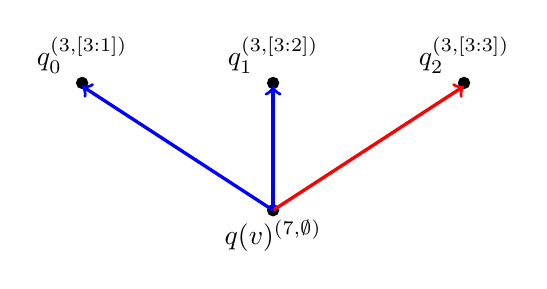
\begin{tikzpicture}[scale=\textwidth/30cm,samples=200]
%%% The nodes represents the k query in the first round
\filldraw[black] (0, 4) circle (5pt) node [anchor=south]{$q_0^{(3,[3:1])}$};
\filldraw[black] (6, 4) circle (5pt) node [anchor=south]{$q_1^{(3,[3:2])}$};
\filldraw[black] (12, 4) circle (5pt) node [anchor=south]{$q_2^{(3,[3:3])}$};
\filldraw[black] (6, 0) circle (5pt) node [anchor=north]{$q(v)^{(7,\emptyset)}$};
\draw[very thick,->, blue] (6, 0)  -- (6, 3.9) ;
\draw[very thick,->, red] (6, 0)  -- (12, 3.9) ;
\draw[very thick,->, blue] (6, 0)  -- (0, 3.9) ;
\end{tikzpicture}
\caption{A query-based dependency graph for two round algorithm complete version}
\label{fig:two-round-graph}
\end{figure}
%\end{figure}
% Even though the high level loop language provides necessary information for static analysis on most real-world data analysis algorithms, it is not suitable to conduct a static analysis directly on. To be specific, it is challenging to achieve a formal definition of the number of rounds of adaptivity for algorithms using the high level language due to the characteristics depicted in its syntax: the execution of one query $q(e)$ in a program $p$ is decided not only by its explicit control flow (e.g. if statement), but also by its argument $e$. 
%
% Then we have the adaptivity calculated from the graph as:
% \[
% \begin{array}{ll}
% A^*(TR, D, m, w) & = \max\limits_{q(v)^{(l,w)},q'(v')^{(l',w')} \in V }\{ |p(q(v)^{(l,w)}, q'(v')^{(l',w')} )| \}\\
% & = |p(q_2^6, q_1^{(3,3)})| = |p(q_2^6, q_1^{(3,1)})| = |p(q_2^6, q_1^{(3,2)})|\\
% & = 1
% \end{array}
% \]
We can notice the complete version generates the similar query-based dependency graph as its simplified version in Figure~\ref{fig:simpl-two-round-graph}.

